\subsection{Modifying the compiler backend}
\label{backend}

First, we had to make a new version of the code generator. The compiler now outputs a JSON file, containing the elements described below.

\begin{itemize}
\item The list of the classes that the program contains
\item For each class, the list of its methods
\item For each method
	\begin{itemize}
	\item the variables declared in it
	\item the arguments list, along with their type
	\item the code
	\end{itemize}
\end{itemize}

The code takes the form of a custom simplified bytecode-like language, whose full specification can be found in the Annex. It is similar to Java's, with several notable differences.

\begin{itemize}
\item variables, methods and classes are referred to by their name, and not a numeric identifier
\item an instruction \textsc{stat} is used to map bytecode instructions to source code lines
% todo
\end{itemize}


%If you are using theoretical concepts, explain them first in this subsection.
%Even if they come from the course (eg. lattices), try to explain the essential
%points \emph{in your own words}. Cite any reference work you used like this
%\cite{TigerBook}. This should convince us that you know the theory behind what
%you coded. 



\subsection{Porting the compiler in the browser}

To make the compiler run in the browser, we used \textsc{ScalaJS}, an EPFL-made library that transcompiles Scala to JavaScript.
\textbf{TODO[Hadrien] Talk about browserFS}
This allows us to conveniently output a JSON file (described in section \ref{subsec:backend}) containing the program structure and code.


\subsection{Implementation of the virtual machine}

At this stage, we had a compiler able to run in the browser and output a custom representation of any Tool program, but nothing to interpret it.
We have implemented a JavaScript virtual machine able to execute instructions that we have defined for our custom bytecode-like language.

\subsubsection{Architecture}

The execution is handled by the Engine class. It contains a StateMachine and methods to handle the debugging control flow (breakpoints, run, step into, etc.).
The state machine contains information about the current state of the program (stack, program counter, current scope...) as well as methods to change it.\\

\begin{figure}[h]
  \centering
    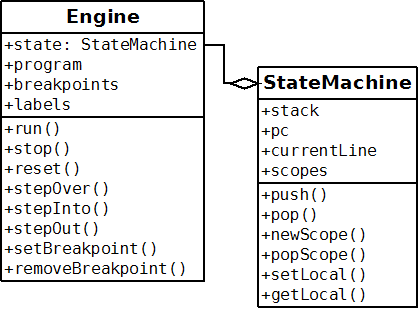
\includegraphics[scale=0.6]{diag.png}
     \caption{(Non-exhaustive) class structure}
\end{figure}

\subsubsection{Control flow}

\textbf{TODO : talk about labels, step in, step out, etc}

\subsection{Developing the web interface}

After that, we had to implement the web interface of the debugger. It is divided into four main parts.

\begin{itemize}
\item The code editor, where you can type code and set breakpoints
\item The toolbar, which allows you to load a Tool source file, compile it, and control the debugging process (run / stop / step over / step into / step out)
\item The console, where you can see messages from the debugger, compilation errors, and the program output
\item The right panel, that allows you to see the values of the variables in the current scope, the call stack and the breakpoints you have set. Clicking on an element of the call stack will bring you at the location the call was made. Breakpoints can be disabled by clicking on the green dot icon, and removed with a right click.
\end{itemize}

The interface was made in HTML and JavaScript, with the use of \href{http://dojotoolkit.org/reference-guide/1.10/dijit/}{Dijit}, a popular library to create web user interfaces.

\subsection{Implementation Details}
Describe all non-obvious tricks you used. Tell us what you thought was hard and
why. If it took you time to figure out the solution to a problem, it probably
means it wasn't easy and you should definitely describe the solution in details
here. If you used what you think is a cool algorithm for some problem, tell us.
Do not however spend time describing trivial things (we what a tree traversal
is, for instance). 

After reading this section, we should be convinced that you knew what you were
doing when you wrote your extension, and that you put some extra consideration
for the harder parts.
